\documentclass[border=12pt]{standalone}
\usepackage[utf8]{inputenc}
\usepackage[T1]{fontenc}
\usepackage{lmodern}
\usepackage{tikz}
\usetikzlibrary{positioning,arrows.meta,fit,backgrounds}

\definecolor{mxNavy}{HTML}{12405E}
\definecolor{mxBlue}{HTML}{2A85BE}
\definecolor{mxBox}{HTML}{EEF7FC}
\definecolor{mxWarn}{HTML}{FFF8EC}
\definecolor{mxGreen}{HTML}{F0FAF4}

\tikzset{
  comp/.style={rectangle, draw=mxBlue, fill=mxBox, thick, rounded corners=3pt, text width=3.55cm, minimum height=1.25cm, align=center, font=\scriptsize\sffamily},
  ext/.style={rectangle, draw=black!55, fill=mxWarn, thick, rounded corners=3pt, text width=3.55cm, minimum height=1.25cm, align=center, font=\scriptsize\sffamily},
  db/.style={rectangle, draw=green!50!black, fill=mxGreen, thick, rounded corners=3pt, text width=3.55cm, minimum height=1.25cm, align=center, font=\scriptsize\sffamily},
  arr/.style={-{Stealth[length=2.2mm]}, thick, color=mxNavy},
  bi/.style={{Stealth[length=2.2mm]}-{Stealth[length=2.2mm]}, thick, color=mxBlue},
  lbl/.style={font=\tiny\sffamily\bfseries, fill=white, inner sep=1.5pt}
}

\begin{document}
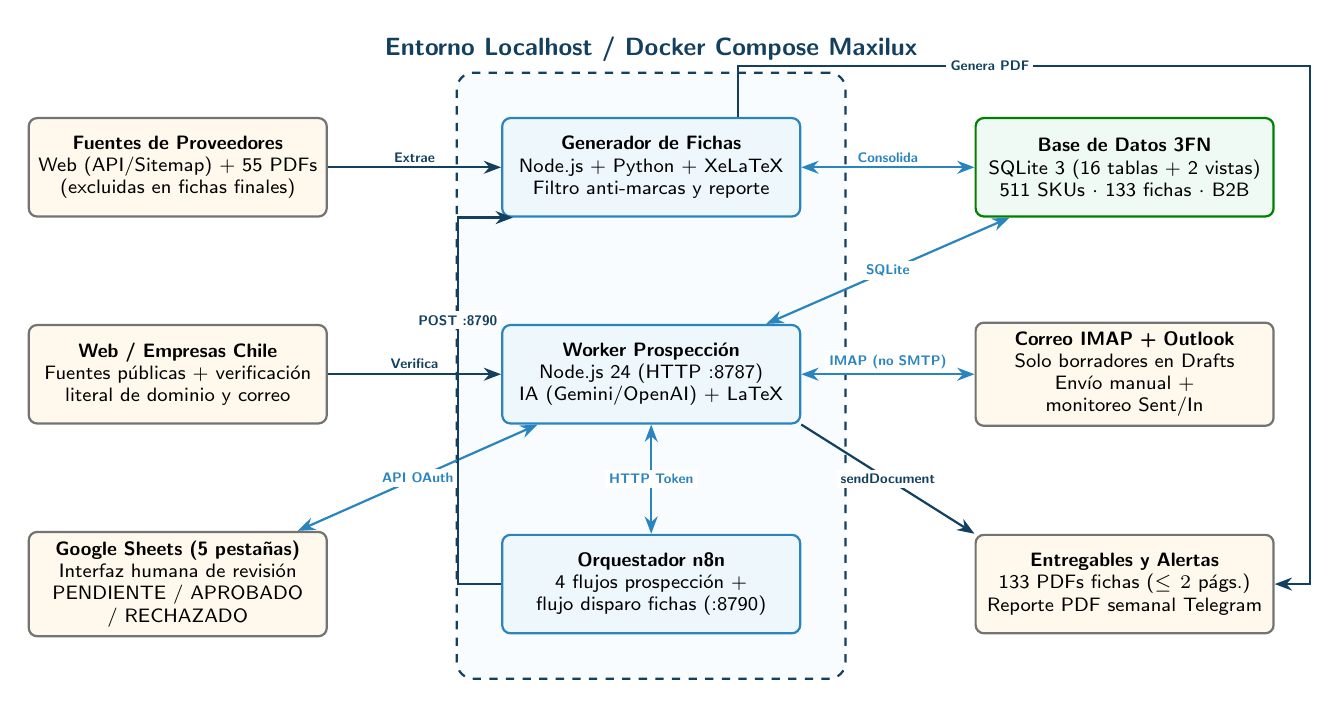
\begin{tikzpicture}[node distance=1.35cm and 2.1cm]

% Capa Fuentes Externas (Izquierda)
\node[ext] (prov) {\textbf{Fuentes de Proveedores}\\Web (API/Sitemap) + 55 PDFs\\(excluidas en fichas finales)};
\node[ext, below=of prov] (webb2b) {\textbf{Web / Empresas Chile}\\Fuentes públicas + verificación\\literal de dominio y correo};
\node[ext, below=of webb2b] (sheets) {\textbf{Google Sheets (5 pestañas)}\\Interfaz humana de revisión\\PENDIENTE / APROBADO / RECHAZADO};

% Capa Automatización y Servicios (Centro)
\node[comp, right=2.2cm of prov] (gen) {\textbf{Generador de Fichas}\\Node.js + Python + XeLaTeX\\Filtro anti-marcas y reporte};
\node[comp, right=2.2cm of webb2b] (worker) {\textbf{Worker Prospección}\\Node.js 24 (HTTP :8787)\\IA (Gemini/OpenAI) + LaTeX};
\node[comp, right=2.2cm of sheets] (n8n) {\textbf{Orquestador n8n}\\4 flujos prospección +\\flujo disparo fichas (:8790)};

% Capa Datos y Salidas (Derecha)
\node[db, right=2.2cm of gen] (bd) {\textbf{Base de Datos 3FN}\\SQLite 3 (16 tablas + 2 vistas)\\511 SKUs $\cdot$ 133 fichas $\cdot$ B2B};
\node[ext, right=2.2cm of worker] (imap) {\textbf{Correo IMAP + Outlook}\\Solo borradores en Drafts\\Envío manual + monitoreo Sent/In};
\node[ext, right=2.2cm of n8n] (tg) {\textbf{Entregables y Alertas}\\133 PDFs fichas ($\le 2$ págs.)\\Reporte PDF semanal Telegram};

% Contenedor Core Localhost / Docker
\begin{scope}[on background layer]
  \node[rectangle, draw=mxNavy, dashed, thick, rounded corners=6pt, fill=mxBox!35, fit=(gen)(worker)(n8n), inner sep=16pt,
        label={[font=\small\bfseries\sffamily, text=mxNavy]above:Entorno Localhost / Docker Compose Maxilux}] (core) {};
\end{scope}

% Conexiones limpias sin cruces
\draw[arr] (prov) -- node[lbl, above]{Extrae} (gen);
\draw[arr] (webb2b) -- node[lbl, above]{Verifica} (worker);
\draw[bi] (sheets) -- node[lbl, midway]{API OAuth} (worker);
\draw[bi] (n8n) -- node[lbl, midway]{HTTP Token} (worker);
\draw[arr] (n8n.west) -- ++(-0.55,0) |- node[lbl, pos=0.36]{POST :8790} (gen.200);
\draw[bi] (gen) -- node[lbl, above]{Consolida} (bd);
\draw[bi] (worker) -- node[lbl, midway]{SQLite} (bd);
\draw[bi] (worker) -- node[lbl, above]{IMAP (no SMTP)} (imap);
\draw[arr] (gen.30) -- ++(0,0.65) -| node[lbl, pos=0.22]{Genera PDF} ([xshift=0.45cm]tg.east) -- (tg.east);
\draw[arr] (worker.south east) -- node[lbl, midway]{sendDocument} (tg.north west);

\end{tikzpicture}
\end{document}
